%!TEX TS-program = xelatex
%!TEX encoding = UTF-8 Unicode
%chktex-file 1

\documentclass[a4paper,11pt,twoside]{book}
% \documentclass[hidelinks,a4paper,11pt,twoside]{book}
\usepackage{upatras-thesis}
\usepackage{tabularx}
\usepackage{subcaption}
\usepackage{bm}
\usepackage{listings}
\usepackage{textcomp}
\usepackage{color}
\usepackage{dirtree}
\lstloadlanguages{C,C++,csh,Java}

\definecolor{red}{rgb}{0.6,0,0} 
\definecolor{blue}{rgb}{0,0,0.6}
\definecolor{green}{rgb}{0,0.8,0}
\definecolor{cyan}{rgb}{0.0,0.6,0.6}
\definecolor{cloudwhite}{rgb}{1.0, 1.0, 1.0}

\lstdefinestyle{sharpc}{
language={[Sharp]C},
basicstyle=\footnotesize\ttfamily,
numbers=left,
numberstyle=\tiny,
numbersep=5pt,
tabsize=2,
extendedchars=true,
breaklines=true,
frame=b,
stringstyle=\color{blue}\ttfamily,
showspaces=false,
showtabs=false,
xleftmargin=17pt,
framexleftmargin=17pt,
framexrightmargin=5pt,
framexbottommargin=4pt,
commentstyle=\color{green},
morecomment=[l]{//}, %use comment-line-style!
morecomment=[s]{/*}{*/}, %for multiline comments
showstringspaces=false,
morekeywords={ abstract, event, new, struct,
as, explicit, null, switch,
base, extern, object, this,
bool, false, operator, throw,
break, finally, out, true,
byte, fixed, override, try,
case, float, params, typeof,
catch, for, private, uint,
char, foreach, protected, ulong,
checked, goto, public, unchecked,
class, if, readonly, unsafe,
const, implicit, ref, ushort,
continue, in, return, using,
decimal, int, sbyte, virtual,
default, interface, sealed, volatile,
delegate, internal, short, void,
do, is, sizeof, while,
double, lock, stackalloc,
else, long, static,
enum, namespace, string, Vector3},
keywordstyle=\color{cyan},
identifierstyle=\color{red},
backgroundcolor=\color{cloudwhite},
}

\lstdefinestyle{sharpframe}{
language={[Sharp]C},
basicstyle=\footnotesize\ttfamily,
numbers=left,
numberstyle=\tiny,
numbersep=5pt,
tabsize=2,
extendedchars=true,
breaklines=true,
frame=tlrb,
stringstyle=\color{blue}\ttfamily,
showspaces=false,
showtabs=false,
xleftmargin=17pt,
framexleftmargin=17pt,
framexrightmargin=5pt,
framexbottommargin=4pt,
commentstyle=\color{green},
morecomment=[l]{//}, %use comment-line-style!
morecomment=[s]{/*}{*/}, %for multiline comments
showstringspaces=false,
morekeywords={ abstract, event, new, struct,
as, explicit, null, switch,
base, extern, object, this,
bool, false, operator, throw,
break, finally, out, true,
byte, fixed, override, try,
case, float, params, typeof,
catch, for, private, uint,
char, foreach, protected, ulong,
checked, goto, public, unchecked,
class, if, readonly, unsafe,
const, implicit, ref, ushort,
continue, in, return, using,
decimal, int, sbyte, virtual,
default, interface, sealed, volatile,
delegate, internal, short, void,
do, is, sizeof, while,
double, lock, stackalloc,
else, long, static,
enum, namespace, string, Vector3},
keywordstyle=\color{cyan},
identifierstyle=\color{red},
backgroundcolor=\color{cloudwhite},
}

\lstdefinestyle{ccin}{
    language={[Sharp]C},
    basicstyle=\ttfamily,
    identifierstyle=\color{cyan}
}

\renewcommand{\lstlistingname}{Κώδικας}
% \usepackage{caption}
% \DeclareCaptionFont{black}{\color{black}}
% \DeclareCaptionFormat{listing}{{\parbox{\textwidth}{\hspace{15pt}#1#2#3}}}
% \captionsetup[lstlisting]{format=plain, labelfont=black,textfont=black, singlelinecheck=false, margin=0pt, font={bf,footnotesize}}

\newcommand{\shortdoctitle}{Διπλωματική Εργασία}
\newcommand{\doctitle}{Ανάπτυξη συστήματος μεικτής πραγματικότητας για υποστήριξη ατόμων με προβλήματα όρασης}
\newcommand{\division}{Ηλεκτρονικής και Yπολογιστών}

\newcommand{\me}{Αγγελου Καρδουτσου του Αποστολου}
\newcommand{\metonoi}{Άγγελου Καρδούτσου του Απόστoλου}

\newcommand{\nomme}{Άγγελος Καρδούτσος του Απόστολου}

\newcommand{\studnum}{1059372}
\newcommand{\keywordsEnglish}{Augmented Reality, Virtual Reality, Mixed Reality, Microsoft HoloLens 2, Microsoft Visual Studio, Unity, spatial mapping, spatial audio, visual impairment, accessibility}
\newcommand{\keywords}{Εκτεταμένη Πραγματικότητα, Επαυξημένη Πραγματικότητα, Μικτή Πραγματικότητα, Microsoft HoloLens 2, Microsoft Visual Studio, Unity, χωρική χαρτογράφηση, χωρικός ήχος, απώλεια όρασης, προσβασιμότητα}
\newcommand{\arximonthyear}{Μάιος 2023}
\newcommand{\telosmonthyear}{Φεβρουάριος 2024}
% To modify
\newcommand{\thesisnum}{XXXX}
\newcommand{\supname}{Νικόλαος Αβούρης}
\newcommand{\suptitle}{Καθηγητής}
\newcommand{\headofdivision}{Γεώργιος Θεοδωρίρης}
\newcommand{\headofdivisiontitle}{Καθηγητής}
\newcommand{\didaktorikosOnoma}{Γεώργιος Παπαδούλης}
% To modify
\newcommand{\imerominiaExetasis}{\ldots\ldots/\ldots\ldots/\ldots\ldots\ldots\ldots}
% To modify
\newcommand{\epitropiEna}{Όνομα Επώνυμο}
% To modify
\newcommand{\epitropiDyo}{Όνομα Επώνυμο}
% To modify
\newcommand{\epitropiEnaTitle}{Βαθμίδα}
% To modify
\newcommand{\epitropiDyoTitle}{Βαθμίδα}

\newcommand{\depECE}{ΗΜ\&ΤΥ}

\setlength{\parindent}{24pt}

\author{\me}

\newcommand{\schema}{Σχήμα}

\newcommand{\code}[1]{\lstinline[style=ccin]{#1}}


% PDF settings
%
\hypersetup{
    pdfauthor={\me},
    pdftitle={\shortdoctitle},
    pdfsubject={\doctitle},
    pdfkeywords={\keywords},
    pdfproducer={XeLaTex},
    pdfcreator={\creator}
}

\begin{document}


\pagenumbering{roman}
%set the number of sectioning levels that get number and appear in the contents
\setcounter{page}{3}

\begin{titlepage}
\begin{center}
% Upper part of the page
\textsc{\textbf{\large ΠΑΝΕΠΙΣΤΗΜΙΟ ΠΑΤΡΩΝ - ΠΟΛΥΤΕΧΝΙΚΗ ΣΧΟΛΗ}\\
\large ΤΜΗΜΑ ΗΛΕΚΤΡΟΛΟΓΩΝ ΜΗΧΑΝΙΚΩΝ\\ΚΑΙ ΤΕΧΝΟΛΟΓΙΑΣ ΥΠΟΛΟΓΙΣΤΩΝ}\\


\includegraphics[width= 0.8\textwidth]{up_landscape}\\  

\textsc{\Large τομέας: \division }\\[1cm]

\textsc{\uline{\LARGE{\shortdoctitle }}}\\ [0.5cm]
του φοιτητή του Τμήματος Ηλεκτρολόγων Μηχανικών και Τεχνολογίας\\
Υπολογιστών της Πολυτεχνικής Σχολής  του Πανεπιστημίου Πατρών\\[1cm]

\textsc{\LARGE \me }\\[0.5cm]
\textsc{\Large αριθμός μητρώου: \studnum}\\[1cm]

\uline{\large Θέμα}\\[0.5cm]
\textbf{\large \doctitle }\\[1cm]
\uline{\large Επιβλέπων}\\[0.5cm]
\large \supname \\[1cm]
\begin{center}
\large{Αριθμός Διπλωματικής Εργασίας: \thesisnum }\hspace{3cm}
\end{center}
\vfill
% Bottom of the page
\large{Πάτρα, \telosmonthyear}
\end{center}
\end{titlepage}

\clearemptydoublepage

\pagestyle{empty}
\begin{center}
{\LARGE ΠΙΣΤΟΠΟΙΗΣΗ\\[1cm]}
\large Πιστοποιείται ότι η διπλωματική εργασία με θέμα\\[1cm]
\textbf{\bf \large \doctitle }\\[1cm]
του φοιτητή του Τμήματος Ηλεκτρολόγων Μηχανικών και Τεχνολογίας Υπολογιστών\\[1cm]
\textbf{\metonoi}\\[0.5cm]
(Α.Μ.: \studnum)\\[1cm]
παρουσιάστηκε δημόσια στο τμήμα  Ηλεκτρολόγων Μηχανικών και Τεχνολογίας Υπολογιστών στις\\[1cm]
\Large{\imerominiaExetasis}\\[1cm]
\large και εξετάστηκε από την ακόλουθη εξεταστική επιτροπή:\\[1cm]
\supname, \suptitle, \uoP\\[0.2cm]
\epitropiEna, \epitropiEnaTitle, \uoP\\[0.2cm]
\epitropiDyo, \epitropiDyoTitle, \uoP\\[1cm]
\end{center}
\begin{minipage}{0.5\textwidth}
\begin{flushleft} \large
Ο Επιβλέπων\\[0.5cm]
\supname\\
\emph{\suptitle}
\end{flushleft}
\end{minipage}
\begin{minipage}{0.5\textwidth}
\begin{flushright} \large
Ο Διευθυντής του Τομέα\\[0.5cm]
\headofdivision\\
\emph{\headofdivisiontitle}
\end{flushright}
\end{minipage}

\clearemptydoublepage

% !TEX root = ../main.tex

\pagestyle{empty}
\begin{center}
\Large{Στοιχεία διπλωματικής εργασίας}\\[1cm]
{\large Θέμα:}
\textbf{\large \doctitle}\\[1cm]
\large {Φοιτητής: \textbf{\nomme}\\[1cm]
\emph{\large{Ομάδα επίβλεψης}}\\[0.3cm]
\textbf{\supname, \suptitle, \uoP}\\
% \textbf{Βαθμίδα και Ονοματεπώνυμο Συνεπιβλέποντα}\\
% \textbf{\didaktorikosOnoma}\\[1cm]
Περίοδος εκπόνησης της εργασίας:\\ {\arximonthyear} - {\telosmonthyear}\\[1cm]
Η εργασία αυτή γράφτηκε στο \XeLaTeX{} και χρησιμοποιήθηκε η γραμματοσειρά GFS Didot του Greek Font Society.}
\end{center}

\clearemptydoublepage

\pagestyle{plain}
\begin{center}
{\LARGE Περίληψη}\\[1cm]
\end{center}

\setlength{\parindent}{0pt}
\textbf{Παράγραφος 1}: Περιγραφή σκοπού διπλωματικής

\textbf{Παράγραφος 2}: Περιγραφή του τι περιγράφουμε στο τεχνολογικό υπόβαθρο και για
την ανάπτυξη της εφαρμογής

\textbf{Παράγραφος 3}: Περιγραφή του πειράματος (τόπος και τρόπος διεξαγωγής, συμμετέχοντες)

\textbf{Παράγραφος 4}: Περογραφή του τελευταίου κεφαλαίου

\textbf{Λέξεις-κλειδιά}: {\keywords}


\clearemptydoublepage

\pagestyle{plain}
\begin{center}
{\LARGE Extensive English Summary}\\[1cm]
\end{center}

\setlength{\parindent}{0pt}
This thesis aims to create an application for the mixed reality device Microsoft HoloLens 2. Its goal is to support individuals with visual impairments, contributing to their independence and accessibility. Specifically, it offers the ability to safely navigate an unfamiliar environment.

Initially, the theoretical and technological background is described. More specifically, we present the causes that lead to vision loss, its impact on the individual, and the available solutions to address it. Additionally, the concepts of virtual, augmented, and mixed reality are explained, and the technical characteristics of the Microsoft HoloLens 2 device and its capabilities, such as spatial mapping and spatial sound, are analyzed, along with the tools used for the application development, such as Unity.

Next, the implementation of the application is presented, starting with its design and the constraints that were set, followed by the way the project was organized and prepared. A detailed description of all the application's functions follows, with the main ones being obstacle detection and user warning, and the way they were developed.

The application evaluation was carried out with the help of ten volunteers, who were asked to test it alongside a widely used tool for visually impaired individuals, the cane. From the tests using both tools by the volunteers, we manage to collect significant comparative data, which are analyzed along with the responses from the questionnaires and the users' observations.

Finally, the thesis was completed by outlining possible future extensions and improvements of the application to provide an even better experience for the end-user.
\\[\baselineskip]
\textbf{Keywords}: {\keywordsEnglish}

\clearemptydoublepage

\begin{center}
{\LARGE Ευχαριστίες}\\[1cm]
\end{center}

\setlength\parindent{24pt}Όσο κι αν φαίνεται σαν ατομική δουλειά η παρούσα εργασία, στην πραγματικότητα βοήθησαν αρκετοί άνθρωποι (ο καθένας με το δικό του τρόπο) για να ολοκληρωθεί. 

\clearemptydoublepage

\pagestyle{fancy}

\tableofcontents
\clearemptydoublepage
\listoffigures
\clearemptydoublepage
\listoftables
\clearemptydoublepage
% \lstlistoflistings
% \clearemptydoublepage

% \mainmatter % book mode only

\pagenumbering{arabic}
\setcounter{page}{1}

\mainmatter
\chapter{Εισαγωγή}\label{ch:introduction}
%!TEX root = ../main.tex

\chapter*{Εισαγωγή}
\markboth{Εισαγωγη}{}
%\vspace{-1.3in}
\lettrine[findent=2pt]{\fbox{\textbf{Η}}}{εργασια} αυτή έχει γίνει προσπάθεια να γραφεί σε ανεξάρτητα κεφάλαια, τα οποία θα δώσουν στον αναγνώστη τις απαιτούμενες γνώσεις ώστε να καταλάβει σε βάθος τις τεχνικές που χρησιμοποιούνται. Σε κάθε κεφάλαιο γίνεται αναλυτική παρουσίαση των τεχνικών καθώς και του υπόβαθρου που πρέπει να έχει κάποιος ώστε τις κατανοήσει, ωστόσο θεωρείται πως ο αναγνώστης έχει ήδη κάποιες γνώσεις στο χώρο της επεξεργασίας σήματος και εικόνας. Έτσι, βασικές έννοιες και μηχανισμοί της ανωτέρω περιοχής θα θεωρούνται δεδομένοι και δε θα γίνει κάποια ανάλυσή τους στο κείμενο αυτό, εκτός αν κρίνεται απαραίτητο.

\clearemptydoublepage

\chapter{Θεωρητικό και Τεχνολογικό Υπόβαθρο}\label{ch:technicalAndTheoreticalBg}
%!TEX root = ../main.tex

Στο παρών κεφάλαιο θα πραγματοποιηθεί μια αναλυτική παρουσίαση του θεωρητικού και τεχνολογικού υπόβαθρου, που αποτέλεσε βάση για την υλοποίηση της εφαρμογής. Αρχικά, θα δοθεί μια εξήγηση για το τι εστί απώλεια όρασης, τι δυσκολίες αντιμετωπίζουν τα άτομα με αυτό το είδος αναπηρίας, καθώς και τις τρέχουσες λύσεις για την καταπολέμηση δυσκολιών προσβασιμότητας (\hyperref[sec:visualImpairment]{Κεφάλαιο~\ref*{sec:visualImpairment}}). Στη συνέχεια, θα δοθεί ο ορισμός της εκτεταμένης πραγματικότητας, καθώς και τις εφαρμογές που βρίσκει στην καθημερινότητα του ανθρώπου (\hyperref[sec:extendedReality]{Κεφάλαιο~\ref*{sec:extendedReality}}). Τέλος, θα δοθεί μια περιγραφή της συσκευής Microsoft Hololens 2 και των λειτουργιών της (\hyperref[sec:hololensDesc]{Κεφάλαιο~\ref*{sec:hololensDesc}}), καθώς και τα εργαλεία, τα οποία θα χρησιμοποιηθούν για την ανάπτυξη της εφαρμογής (\hyperref[sec:hololensTools]{Κεφάλαιο~\ref*{sec:hololensTools}}).

\section{Όραση}\label{sec:visualImpairment}
\subsection{Τρόπος Λειτουργίας}\label{subsec:visionDefinition}
Η όραση αποτελεί μία από τις βασικές αισθήσεις του ανθρώπου. Η αίσθηση αυτή βασίζεται στη λειτουργία του ματιού, το οποίο αποτελεί το αισθητήριο όργανο και στο εσωτερικό του οποίου εισερχεται το φως, διαπερνώντας αρχικά το κερατωειδή χιτώνα και την κόρη και προσπίπτει, τελικά, στον αμφιβληστορειδή χιτώνα (\hyperref[fig:eye_anatomy]{\schema~\ref*{fig:eye_anatomy}}). Αυτό οδηγεί σε διέγερση των οπτικών νεύρων και τα οπτικά σήματα, που αποστέλλονται στον εγκέφαλο, μετατρέπονται σε εικόνα~\cite{nationaleyeinstitute_2022_how}\cite{anspaugh_2022_vision}.

\begin{figure}[!h]
  \centering
  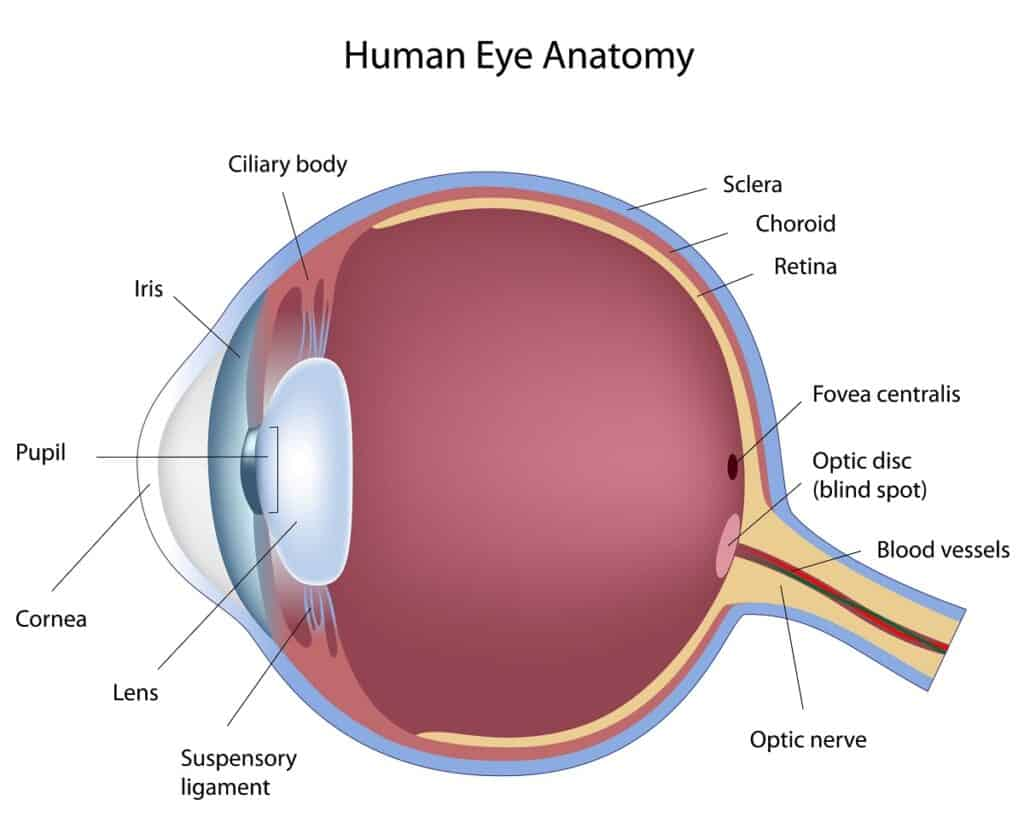
\includegraphics[width=90mm]{images/eye_anatomy.jpg}
  \caption{Η ανατομία του ματιού {\footnotesize(Πηγή: dreamstime.com)}}\label{fig:eye_anatomy}
\end{figure}

\subsection{Απώλεια Όρασης: Κατηγοροποίηση και Αιτίες}\label{subsec:visionCauses}
Όταν η φυσιολογική λειτουργία του αισθητήριου οργάνου διαταραχθεί, τότε το άτομο έρχεται αντιμέτωπο με κάποιο τύπο προβλήματος όρασης. Με βάση τον Παγκόσμιο Οργανισμό Υγείας (Π.Ο.Υ.), τα άτομα αυτά κατηγοροποιούνται σε 6 κατηγορίες (Κατηγορία 0 έως Κατηγορία 5), ανάλογα την οπτική τους οξύτητα, δηλαδή της ικανότητάς του να διακρίνουν σχήματα και λεπτομέρειες από κάποια δεδομένη μακρυμένη απόσταση:
\begin{itemize}
    \item Στην κατηγορία 0 ανήκουν άτομα με με πλήρως ή σχεδόν πλήρως λειτουργική όραση
    \item Στην κατηγορία 1 και 2 ανήκουν άτομα που έχουν υποστεί μερική απώλεια της όρασής τους
    \item Τέλος, στις κατηγορίες 3, 4 και 5 εντάσσονται τα άτομα με σχεδόν πλήρη ή πλήρη απώλεια όρασης
\end{itemize}
Αντιθέτως, για κοντινές αποστάσεις, τα άτομα με προβλήματα όρασης εντάσσονται σε μία μόνο κατηγορία~\cite{worldhealthorganization_2019_world}.

Οι κυριότερες αιτίες, οι οποίες προκαλούν προβλήματα όρασης, απότελουν:
\begin{itemize}
    \item τα διαθλαστικά σφάλματα
    \item ο καταρράκτης
    \item η διαβητική αμφιβληστροειδοπάθεια
    \item το γλαύκωμα
    \item η ηλικιακή εκφύλιση της ωχράς κηλίδας
\end{itemize}
Από τα ανωτέρω, η κυριότερη αίτια πλήρης απώλειας όρασης σε άτομα ηλικίας 50 ετών και άνω αποτελεί ο καταράκτης, σε ποσοστό 46\% των ατόμων που υπέστησαν πλήρη απώλεια όρασης το 2020. Αντιθέτως, για την ίδια ηλικία ομάδα, η οποία αντιμέτωπιζε μερική απώλεια όρασης, κύριες αιτίες αποτελούν τα υποδιορθωμένα διαθλαστικά σφάλματα και ο καταράκτης, σε ποσοστό 30\% το καθένα για το ίδιο έτος~\cite{adelson_2021_causes}.

\subsection{Απώλεια Όρασης: Αντίκτυπος}\label{subsec:visionImpact}
Η απώλεια όρασης έχει ιδιαίτερο αντίκτυπο στην προσωπική, κοινωνική και οικονομική ζωή του ατόμου, ανεξαρτήτου της ηλικίας του. Η εκπλήρωση απλών καθημερινών εργασιών μπορεί να αποδειχθεί ιδιαίτερα δύσκολη και χρόνοβορα, επειδυνώνοντας ιδαίτερα την ποιότητα ζωής του ατόμου~\cite{west_2002_how}\cite{khorraminejad_2016_the}, ακόμη και σε επίπεδο χαμηλότερο από αυτό ατόμων που αντιμετωπίζουν χρόνια νοσήματα~\cite{langelaan_2007_impact}.



Η εμφάνιση προβλημάτων όρασης σε αρκετά νεαρή ηλικία μπορεί να επηρέασει αισθητά την ανάπτυξη ικανοτήτων όπως είναι η κινητήρια και η γνωστική του ικανότητα και η κοινωνική του καλλιέργεια~\cite{worldhealthorganization_2023_blindness}. Αντιθέτως, στην ενήλικη ζωή του, μπορεί να δυσκολέψει την εύρεση εργασίας και να επηρεάσει την ψυχική του υγεία, προκαλώντας μέχρι και άγχος και κατάθλιψη~\cite{khorraminejad_2016_the}. Τέλος, σε άτομα άρκετα μεγάλης ηλικίας, η απώλεια όρασης μπορεί να δυσχεράνει βασικές λειτουργίες, όπως είναι το περπατήμα με εγγενές κίνδυνο την πτώση και τον τραυματισμό~\cite{worldhealthorganization_2023_blindness}.

\subsection{Απώλεια Όρασης: Λύσεις}\label{subsec:visionSolutions}
Πλήθος λύσεων είναι διαθέσιμες στο μέσο άνθρωπο, οι οποίες στοχεύουν στην πρόληψη της απώλειας της όρασης ή στην επιδιόρθωση αυτής. Σε απλές περιπττώσεις, όπως είναι η μυωπία, πρεσβυωπία, κ.λ.π., το πρόβλημα μπορεί να επιλύεται με χρήση διορθωτικών φακών ή εγχείρηση στο αισθητήριο όργανο~\cite{worldhealthorganization_2023_blindness}. Επίσης, για άτομα που δεν μπορούν επιδιορθώσουν το πρόβλημα όρασής του, έχουν αναπτυχθεί συσκευές και τεχνολογίες, οι οποίες συνεχώς εξελίσσονται και έχουν ως σκοπό την εξυπηρέτηση του ατόμου σε διάφορες πτυχές της καθημερινότητάς του. Επί δεκαετείες, το μπαστούνι αποτελεί μια αρκετά διαδεμένη συσκευή, που βοηθά ένα άτομο να αναγνωρίζει εμπόδια, καθώς περιηγείται σε έναν χώρο. Σε συνδυασμό με την απτική πλακόστρωση (\hyperref[fig:tactile_paving]{\schema~\ref*{fig:tactile_paving}}), το άτομο μπορεί να περιηγηθεί σε δημοσίο χώρο, όντας συνεχώς ενήμερος για την ύπαρξη εμποδίων, όπως δρόμοι, διάβαση πεζών, γραμμές τραμ, στη διαδρομή του, ανάλογα με το μοτίβο των πλακών του πεζοδρομίου~\cite{mashiata_2022_towards}.
\begin{figure}[!h]
  \centering
  \includegraphics[width=60mm]{images/tactile-paving.jpg}
  \caption{Απτική πλακόστρωση {\footnotesize(Πηγή: vecteezy.com)}}\label{fig:tactile_paving}
\end{figure}\\
Ευρέως διαδεδομένη είναι και η χρήση σκύλων-βοηθών, οι οποίοι είναι ειδικά εκπαιδευμένοι σχετικά με την αναπηρία του ιδιοκτήτη τους με σκοπό να τους εξυπηρετήσουν στις ιδιαίτερες ανάγκες που μποροί να έχουν. Στην περίπτωση των ατόμων με προβλήματα όρασης, σκοπός τους είναι να κατευθήνουν τον ιδιοκτήτης τους στο προορισμό τους, ειδοποιώντας τον για πιθανά εμπόδια~\cite{illinoisuniversitylibrary_2013_libguides}. Τέλος, αναπτύχθηκε το σύστημα γραφής Braille, ώστε να είναι εφικτή η ανάγνωση κειμένων με τη βοήθεια της αφής.

Στη σύγχρονή εποχή, όλο και περισσότερες συσκεύες κατασκευάζονται λαμβάνοντας εκ των προτέρων υπόψη τη δυνατότητα χρήσης αυτών από άτομα με περιορισμένη όραση. Οι κινητές συσκευές διαθέτουν λογισμικό screen reader (π.χ. TalkBack σε Android συσκεύες ή VoiceOver σε iOS συσκευές), διευκολύνοντας την πλοήγηση του χρήστη στις εφαρμογές του κινητού, καθώς πραγματοποιούν καταγραφή και αναγνώριση των κειμένων και των λειτουργιών, που βρίσκονται στην οθόνη τη δεδομένη χρονική στιγμή, και ο χρήστης, με συγκεκριμένες χειρονομίες, επιλέγει αν επιθυμεί την ανάγνωση κάποιο κειμένου με χρήση text-to-speech ή την πραγματοποίηση κάποιας ενέργειας~\cite{americanfoundationfortheblind_2019_screen}. Επιπλέον, η γλώσσα προγραμματισμού HTML δίνει τη δυνανότητα στους προγραμματιστές να κατασκευάσουν ιστοσελίδες, οι οποίες θα είναι προσβάσιμες από άτομα με περιορισμένη όραση, καθώς οι screen readers θα μπορούν να αναγνωρίζουν τμήματα της ιστοσελίδας, όπως επικεφαλίδες, υπερσυνδέσμους, κουμπιά και το σκοπό που επιτελούν~\cite{w3schools_2020_html}.

Όσον αφορά την περιήγηση ατόμων σε ανοιχτούς ή κλειστούς χώρους, πληθώρα συσκευών έχουν κατασκευαστεί, οι οποίες βελτιώνουν ήδη υπάρχουσες ή προσφέρουν έναν εναλλακτικό τρόπο λειτουργίας και παροχής βοήθειας. Παραδείγματα τέτοιων συσκευών αποτελούν:
\begin{itemize}
  \item \textbf{biped}: Συσκευή, η οποία φοριέται γύρω από το λαιμό του χρήστη. Διαθέτει 3 κάμερες, που προσφέρουν πεδίο ορατότητας 170\textdegree, και ενσωματώνουν λογισμικό για τον εντοπισμό και αναγνώριση εμποδίων. Ο χρήστης προειδοποιείται για εμπόδια με μια ηχητική προειδοποίηση.~\cite{biped}
  \item \textbf{OrCam MyEye}: Φορητή συσκευή, η οποία προσφέρει τη δυνατότητα ανάγνωσης κειμένων, αναγνώρισης αντικειμένων, χρωμάτων και προσώπων.~\cite{ghebali_2023_orcam}
  \item \textbf{BlindSquare}: Εφαρμογή πλοήγησης, η οποία παρέχει αναλύτικες οδηγίες στο χρήστη, ώστε να κατευθυνθεί στο προόρισμο του, παρέχοντας παράλληλα πληροφορίες για το περιβάλλον του χρήστη και για σημεία ενδιαφέροντος.~\cite{blindsquare}
  \item \textbf{Be My Eyes}: Εφαρμογή, η οποία επιτρέπει σε χρήστες να έρθουν σε επικοινωνία με εθελοντές μέσω βιντεοκλήσης, με σκοπό να ζητήσουν βοήθεια.~\cite{a2019_be}
  \item \textbf{WeWALK}: Αποτελεί ένα εξάρτημα για μπαστούνια, το οποίο έχει τη δυνατότητα να εντοπίζει εμπόδια σε χαμηλό ύψος με χρήση υπερήχων και να ειδοποιεί το χρήστη με δονήσεις και ήχο.~\cite{wewalk}
  \item \textbf{Seeing AI}: Εφαρμογή της Microsoft, η οποία, με χρήση τεχνητής νοημοσύνης, παρέχει περιγραφές των αντικειμένων, χρωμάτων, ανθρώπων και κειμένων, τα οποία στοχεύει ο χρήστης με την κάμερα του κινητού του τηλεφώνου.~\cite{seeing}
\end{itemize}

%=========================================

\section{Εκτεταμένη Πραγματικότητα}\label{sec:extendedReality}
Ορισμός\\
Τρέχουσες χρήσεις\\
Συσκευές που παρέχουν αυτές τις δυνατότητες

\subsection{Εικονική Πραγματικότητα}

\subsection{Επαυξημένη Πραγματικότητα}

\subsection{Μικτή Πραγματικότητα}

%=========================================

\section{Hololens}\label{sec:hololensDesc}

\subsection{Περιγραφή Συσκευής}
Description of the device

\subsection{Τεχνικά Χαρακτηριστικά}
Hololens features

\subsection{Τρόποι Αλληλεπίδρασης}
Τρόποι αλληλεπίδρασης

\subsection{Spatial Mapping}

\subsection{Spatial Audio}

%=========================================

\section{Εργαλεία ανάπτυξης για Hololens}\label{sec:hololensTools}

\subsection{Unity}
Περιγραφή περιβάλλοντος

\subsection{Microsoft Visual Studio}
Μικρή περιγραφή της χρήσης του

\subsection{Mixed Reality Toolkit}

%=========================================
\clearemptydoublepage

\chapter{Η υλοποίηση}\label{ch:implementation}
%!TEX root = ../main.tex

Σκοπός του κεφαλαίου αποτελεί η παρουσίαση της διαδικασίας ανάπτυξης της εφαρμογής για τη συσκευή Microsoft HoloLens 2. Πιο συγκεκριμένα, θα παρουσιάσουμε αρχικά τον κύριο στόχο της εφαρμογής, ποιος είναι ο σκοπός που εξυπηρέτει και σε ποιο πρόβλημα προσπαθεί να προσφέρει λύση (\hyperref[sec:appScenario]{Κεφάλαιο~\ref*{sec:appScenario}}). Έπειτα, θα γίνει αναφορά στις αποφάσεις που λήφθηκαν κάτα την σχεδίαση και υλοποίηση της εφαρμογής με βάση και τους περιορισμούς που τέθηκαν (\hyperref[sec:appDesignAndLimitations]{Κεφάλαιο~\ref*{sec:appDesignAndLimitations}}), ενώ θα δοθεί και μια αναλυτική περιγραφή της διαδικασίας υλοποίησης της εφαρμογής και επεξήγηση του κώδικα που αναπτύχθηκε (\hyperref[sec:appImplementation]{Κεφάλαιο~\ref*{sec:appImplementation}}). Το κεφάλαιο θα ολοκληρωθεί παρουσιάζοντας όλες τις κύριες λειτουργίες, οι οποίες αναπτύχθηκαν για την εφαρμογή (\hyperref[sec:appFunctionalities]{Κεφάλαιο~\ref*{sec:appFunctionalities}}).

%TODO: Εναλλακτικός τίτλος: Περιγραφή/Λειτουργίες Εφαρμογής
\section{Σενάριο Εφαρμογής}\label{sec:appScenario}
Στόχος εφαρμογής\\
Περιγραφή σεναρίου χρήσης εφαρμογής

\section{Σχεδιασμός και Περιορισμοί}\label{sec:appDesignAndLimitations}
Κατά τον σχεδιασμό της εφαρμογής, καθώς και κατά τη διάρκεια υλοποίησης αυτής, υπήρξαν πληθώρα περιπτώσεων, όπου κληθήκαμε να λάβουμε ιδιαίτερα σημαντικές αποφάσεις, που επηρέασαν σημαντικά την πορεία ανάπτυξης, λόγων των συνθηκών και προδιαφραφών που τέθηκαν ή των περιορισμών και δυσκολιών που αντιμετωπίσαμε.

Αρχικά, όσον αφορά την προετοιμασία και την εγκατάσταση των εργαλείων, ήρθαμε αντιμέτωποι με ένα ιδιαίτερα λειψό εγχειρίδιο (documentation)~\cite{hferrone_mixed}, το οποίο παρέχει η Microsoft.
Ειδικότερα, το documentation είναι πλούσιο σε πληροφοριές, που βοηθούν προγραμματιστές, οι οποίοι έρχονται πρώτη φορά σε επαφή με το headset, να κατανοήσουν πλήρως έννοιες και τεχνολογίες που αξιοποοιούνται από τη συσκευή, καθώς και τον τρόπο λειτουργίας της. Ωστόσο, σε προγραμματιστικό επίπεδο, οι πληροφορίες είναι ελάχιστες, ενώ οι επεξηγήσεις αντικειμένων, κλάσεων και συναρτήσεων είναι ιδιαίτερα ελλιπείς, καθώς περιορίζονται σε επιδερμικές περογραφές αυτών και την παρουσιασή παραδειγμάτων και σε ένα πολύ μικρό δείγμα αυτών.
Παράλληλα, η Microsoft παρέχει μαθήματα (courses) για την πρακτική εκμάθηση των προγραμματιστών στην ανάπτυξη εφαρμογών για τη συσκεύη με τη χρήση του περιβάλλοντος Unity. Όμως, και σε αυτή την περίπτωση, τα courses περιορίζονται στη χρήση έτοιμων projects, όπου η μόνη συμβολή του χρήστη στη ανάπτυξη αυτών είναι η αλλαγή ορισμένων απλών ρυθμίσεων. Επομένως, κατά τη διάρκεια της ανάπτυξης (development), αναγκαστήκαμε να καταφύγουμε σε οδηγούς (tutorials) και forums, τα οποία αναπτύχθηκαν από τρίτους, από κοινότητες προγραμματιστών που διέθεταν εμπειρία πάνω στη συγκεκριμένη τεχνολογία.
Τέλος, ιδιαίτερο πρόβλημα αποτέλεσε η ασυμβατότητα (incompatibility) μεταξύ των διαφορετικών εκδόσεων των εργαλείων που χρησιμοποιήθηκαν (Unity, MRTK, Visual Studio), το οποίο καθυστέρησε την έναρξη της φάσης ανάπτυξης (development phase).

Επιπλέον, λόγω της ιδιαιτερότητας των χρηστών προς τους οποίους απευθύνεται η εφαρμογή, εκ πρώτης όψεως, φαίνεται αρκέτα οξύμωρη η επιλογή μίας συσκευής που ενσωματώνει την τεχνολογία Μικτής Πραγματικότητας, όπου, επί τον πλείστον, οι εφαρμογές απαιτούν από τους χρήστες να αλληλεπιδράσουν με εικονικά αντικείμενα και η όραση αποδεικνύεται εξαιρετικά σημαντική. Παρ' όλα αυτά, η συσκευή επιλέχθηκε λόγω compact σχεδιασμού, ενσωματώνοντας πληθώρα αισθητήρων σε μια μικρή, φορητή συσκευή. Επίσης, ο προγραμματιστής έχει τη δυνατότητα να ενσωματώσει φωνητικές εντολές, όπου οι χρήστες μπορούν χρησιμοποιήσουν για να αλληλεπιδράσουν με τις λειτουργίες της εφαρμογής.

Πέρα από τις δυνατότητες που προσφέρει η συσκευή, καθιστώντας την ιδανική επιλογή, θέτει, παράλληλα, έχει και ορισμένους περιορισμούς. Συγκεκριμένα, οι περιορισμοί αφορούν τις συνθήκες του περιβάλλοντος, όπου χρησιμοποιείται η συσκευή~\cite{dorreneb_2022_hololens}. 
Για την αποδοτική λειτουργία της συσκευής, πρέπει ο χώρος να είναι καλά φωτιζόμενος, να μην είναι ιδιαίτερα απλός, αλλά, αντιθέτως, να διαθέτει πολλά, μοναδικά αντικειμένα, τα οποία θα εξυπηρετήσουν στην καλύτερη αναγνώριση των αντικειμένων και των εμποδίων κατά τη χωρική χαρτογράφηση. Τέλος, οι συχνές αλλαγές και μετακινήσεις στο χώρο, καθώς και η ύπαρξη ανακλαστικών επιφανειών μπορούν να επηρεάσουν αρνητικά το tracking και τη χαρτογράφηση της συσκευής.
Για τους ανωτέρω λόγους, αποφασίστηκε η χρήση της εφαρμογής να περιοριστεί σε εσωτερικούς χώρους.

% Αδυναμία ανθρώπου να αντιληφθεί προέλευση ήχου στον κάθετο άξονα

\section{Υλοποίηση}\label{sec:appImplementation}
Η υλοποίηση της εφαρμογής, τμηματοποιημένη

\section{Λειτουργίες Εφαρμογής}\label{sec:appFunctionalities}
Τρόπος χρήσης της εφαρμογής

% \begin{theorem}[Shannon-Nyquist]
% 	\label{thrm:shannon-nyquist}
% 	Ένα σήμα με μέγιστη συχνότητα $f_{max}$ μπορεί να ανακτηθεί από τα δείγματά του, αν αυτά ληφθούν με συχνότητα $f_s>2f_{max}$, ή αλλιώς με περίοδο $T_s<\frac{1}{2f_{max}}$. \cite{proakis_sampling}
% \end{theorem}
\clearemptydoublepage

\chapter{Αξιολόγηση}\label{ch:experiment}
%!TEX root = ../main.tex

Σκοπός της αξιολόγησης (γιατί κάνουμε αξιολόγηση)\\
Συυμμετέχοντες\\
Προδιαγραφές (πως προετοιμαστήκαμε με τους εθελοντές για την αξιολόγηση)\\
Ερωτηματολόγια που χρησιμοποιήθηκαν


\section{Διαδικασία/Περιγραφή Πειράματος}
Τρόπος/συνθήκες διεξαγωγής\\
Πιθανοί περιορισμοί

\section{Αποτελέσματα}
Παρατηρήσεις\\
Απαντήσεις ερωτηματολογίου

% \begin{equation} \label{eq:hrmodel}
% \bm{Y}_i=\bm{S}_i\bm{T}_i\bm{H}_i\bm{X}+\bm{n}_i
% \end{equation}

% \begin{algorithm}
%  \KwData{$\bm{dx}$, $\bm{dy}$, $\bm{Y}_i$, $N$, $W$, $\bm{H}$, $S$}
%  \KwOut{High resolution reconstructed $\bm{X}$}
%  $\bm{X} \gets 0$\; 
%  \For{$n \gets 1$ \textbf{to} $N$}{
%  	$\bm{\tilde{Y}} \gets \bm{Y}_i$\;
%     $\bm{i} \gets 1:W/S$\;
%     $\bm{j} \gets 1:H/S$\;
%     $\bm{px}=\bm{i}*S+\bm{dx}_n$\;
%     $\bm{py}=\bm{j}*S+\bm{dy}_n$\;
%     $\bm{X}_{px,py}=\bm{\tilde{Y}}_{i,j}$\;
%     }
%     %\vspace{-1.5em}
%  \caption{Ανακατασκευή shift-add fusion}\label{algo:sr_fusion}
% \end{algorithm}

\clearemptydoublepage

\chapter{Προεκτάσεις και Επίλογος}\label{ch:epilogue}
%!TEX root = ../main.tex

\section{Μελλοντικές προεκτάσεις}\label{sec:futureImprovements}
Ο κύριος στόχος της διπλωματικής εργασίας ήταν η υλοποίησης μιας εφαρμογής, η οποία θα προσέφερε ουσιαστική βοήθεια σε άτομα με προβλήματα όρασης	στην περιήγηση τους σε έναν άγνωστο χώρο. Η ανάπτυξή της βασίζεται στην αξιοποίηση σύγχρονων τεχνολογιών, όπως είναι η Μικτή Πραγματικότητα, η οποία, μέχρι και σήμερα, δεν έχει καταφέρει να εισέλθει σε μεγάλο βαθμό στην καθημερινότητα του μέσου ανθρώπου. Η χρήση της συσκευής Microsoft HoloLens 2 αποτέλεσε ιδανική επιλογή, διότι διαθέτει πληθώρα αισθητήρων απαραίτητων για τους σκοπούς της εφαρμογής μας σε μια φορητή συσκευή, μικρού σχετικά σχετικά μεγέθους. Έτσι μπορέσαμε να επικεντρωθούμε στην ανάπτυξη λογισμικού χωρίς να υπάρχει η ανάγκη δημιουργίας εξειδικευμένου hardware. Επιπλέον, αποτελεί ευκαιρία ώστε άτομα με προβλήματα όρασης να βιώσουν - εν μέρει - την εμπειρία της Μικτής Πραγματικότητας, η οποία γίνεται περισσότερο προσβάσιμη προς αυτούς. %chktex-file 8

Η εφαρμογή, η οποία δημιουργήθηκε, διαθέτει τις απαραίτητες λειτουργίες, ώστε να αποτελέσει ένα πρωτότυπο και να παρουσιαστεί η χρηστικότητά της, ωστόσο βρίσκεται σε ένα αρχικό στάδιο ανάπτυξης. Ιδιαίτερη σημαντική κρίνεται η βελτίωση των προειδοποιητικών ήχων, το οποίο θα βελτίωνε δραματικά την εμπειρία των χρηστών. Επιπλέον, η εφαρμογή επιδέχεται πλήθος αναβαθμίσεων, οι οποίες θα μπορούσαν να βελτιώσουν την απόδοσή της, καθώς και την εμπειρία του χρήστη. Μεταξύ των άλλων, μεγαλύτερο ενδιαφέρον παρουσιάζει η χρήση τεχνητής νοημοσύνης σε συνδυασμό με υπολογιστική όραση με σκοπό, όχι μόνο τον καλύτερο εντοπισμό εμποδίων, αλλά και για την πρόβλεψη πιθανών συγκερούσεων όπως και για την αναγνώριση αντικειμένων και εμποδίων. Προσφέροντας στο χρήστη τη γνώση για το εμπόδιο που βρίσκεται στο δρόμο του, δηλαδή αν πρόκειται για ένα τοίχο, μια καρέκλα, έναν άνρθωπο ή μια πόρτα, του δίνεται η δυνατότητα να προσαρμόσει ανάλογα τον τρόπο αντιμετώπισης αυτής της δυσκολίας, καθώς και να κινείται με μεγαλύτερη ελευθερία στο χώρο, γνωρίζοντας τι υπάρχει σε αυτόν ή από που να μεταβεί σε κάποιο άλλο χώρο. Επίσης, χρήσιμη θα ήταν η δυνατότητα σύνδεσης του κινητού τηλεφώνου του χρήστη με την εφαρμογή μέσω ενός companion app, καθιστώντας τη διαχείριση αυτής και των λειτουργιών της ευκολότερη λόγω των επιλογών προσβασιμότητας που προσφέρει, όπως είναι οι screen readers. Με αυτό τον τρόπο, ο χρήστης δε θα χρειάζεται να βασίζεται αποκλειστικά στη χρήση φωνητικών εντολών. Παράλληλα, το κινητο μπορεί ακομή να προσφέρει απτική ανάδραση και να ενημερώνει το χρήστη, όταν πλησιάζει αρκέτα σε κάποιο εμπόδιο.
% Παράλληλα, θα μπορούσε να λειτουργεί σα συσκευή μετάδοσης του haptic feedback

\section{Επίλογος}\label{sec:conclusion}
\clearemptydoublepage

\backmatter
\bibliography{thesisBibliography} 
\bibliographystyle{IEEEtran}
% %!TEX root = ./main.tex

\begin{thebibliography}{99}

\bibitem{c1} S. C. Park, M. K. Park, and M. G. Kang, “Super-resolution image reconstruction:
A technical overview,” IEEE Signal Processing Magazine, vol. 20, no. 3, pp. 21–36,
May 2003.
\bibitem{keren} D. Keren, S. Peleg, and R. Brada, “Image sequence enhancement using subpixel
displacements,” in IEEE Computer Society Conference on Computer Vision and
Pattern Recognition, June 1988, pp. 742–746.
\bibitem{hardie} R. Hardie, K. Barnard, and E. Armstrong, “Joint MAP registration and high resolution image estimation using a sequence of undersampled images,” IEEE Transactions on Image Processing, vol. 6, no. 12, pp. 1621–1633, December 1997.
\bibitem{patti} A. Patti, M. Sezan, and A. Tekalp, “High-resolution image reconstruction from
a low-resolution image sequence in the presence of time-varying motion blur,” in
Proceedings of the IEEE International Conference on Image Processing, Austin,
TX, vol. 1, 1994, pp. 343–347.
\bibitem{hardie2} R. C. Hardie, K. J. Barnard, J. G. Bognar, E. E. Armstrong, and E. A. Watson, “High resolution image reconstruction from a sequence of rotated and translated
frames and its application to an infrared imaging system,” Optical Engineering,
vol. 37, no. 1, pp. 247–260, January 1998.
\bibitem{alam} M. S. Alam, J. G. Bognar, R. C. Hardie, and B. J. Yasuda, “Infrared image registration and high-resolution reconstruction using multiple translationally shifted aliased video frames,” IEEE Transactions on Instrumentation and Measurement, vol. 49,
no. 5, pp. 923–915, October 2000.
\bibitem{tsai} R. Y. Tsai and T. S. Huang, “Multiframe image restoration and registration,” in Advances in Computer Vision and Image Processing: Image Reconstruction from Incomplete Observations, T. S. Huang, Ed., vol. 1. London: JAI Press, 1984, pp. 317–339.
\bibitem{kim} N. K. Bose, H. C. Kim, and H. M. Valenzuela, “Recursive total least squares algorithm for image reconstruction from noisy undersampled frames,” Multidimensional Systems and Signal Processing, vol. 4, no. 3, pp. 253–268, July 1993.
\bibitem{yang} J. Yang, J. Wright, T. Huang, and Yi Ma. Image super-resolution via sparse representation. IEEE Transactions on Image Processing (TIP), vol. 19, issue 11, 2010.
\bibitem{ransac} Martin A. Fischler and Robert C. Bolles (June 1981). “Random Sample Consensus: A Paradigm for Model Fitting with Applications to Image Analysis and Automated Cartography”. Comm. of the ACM 24 (6): 381–395
\bibitem{wired_ff_algo} Jordan Ellenberg, ”Fill in the Blanks: Using Math to Turn Lo-Res Datasets Into Hi-Res Samples”, 22 February 2010, Wired Magazine \url{http://www.wired.com/2010/02/ff_algorithm/}
\bibitem{incoherence} D.L. Donoho and X. Huo, “Uncertainty principles and ideal atomic decomposition,” IEEE Trans. Inform. Theory, vol. 47, no. 7, pp. 2845–2862, Nov. 2001.
\bibitem{candes} E. Candes, “Compressive sensing,” in Proceedings of the International Congress of Mathematicians, vol. 3, pp. 1433–1452, 2006.
\bibitem{donoho} D. L. Donoho, “Compressed sensing,” IEEE Transactions on Information Theory, vol. 52, no. 4, pp. 1289–1306, 2006.
\bibitem{proakis_sampling} John G. Proakis, Dimitris G. Manolakis , “Digital Signal Processing - Principles, Algorithms, Implementations” 4th edition (Pearson International Edition), Pearson Education, Chapter 1.4.2: The Sampling Theorem 
\bibitem{gonzalez_2d_fft} Rafael C. Gonzalez, Richard E. Woods , “Digital Image Processing” 3rd edition (Pearson International Edition), Pearson Education, Chapter 1.4.2: The 2D Discrete Fourier Transform and its Inverse
\bibitem{shift_add_fusion} S. Farsiu, M. Elad, P. Milanfar, “Fast and Robust Multiframe Super Resolution” IEEE Transactions on Image Processing, vol. 13, no. 10, October 2004
\bibitem{imregintro} ”Image Registration", in Wikipedia: The Free Encyclopedia; (Wikimedia Foundation Inc., updated 2 December 2014, 15:50 UTC) \url{http://en.wikipedia.org/wiki/Image_registration}
\bibitem{cs_intro} M. Davenport, M. Duarte, Y. Eldar, G. Kutyniok, ”Introduction to Compressed Sensing”, Stanford University - Department of Statistics
\bibitem{convexmin} F. Bach, R. Jenatton, J. Mairal, G. Obozinski, ”Convex Optimization with Sparsity-Inducing Norms”, Institut National de Recherche en Informatique et en Automatique (INRIA)
\bibitem{red_dict} H. Rauhut, K. Schnass, and P. Vandergheynst, “Compressed sensing and redundant dictionaries,” IEEE Transactions on Information Theory, vol. 54, no. 5, May 2008.
\bibitem{denoising_dict} M. Elad and M. Aharon, “Image denoising via sparse and redundant representations over learned dictionaries,” IEEE Transactions on Image Processing, vol. 15, pp. 3736–3745, 2006.
\bibitem{im_vid_rest} J. Mairal, G. Sapiro, and M. Elad, “Learning multiscale sparse representations for image and video restoration,” Multiscale Modeling and Simulation, vol. 7, pp. 214–241, 2008.
\bibitem{ksvd_dict} M. Aharon, M. Elad, and A. Bruckstein, “K-SVD: An algorithm for designing overcomplete dictionaries for sparse representation,” IEEE Transactions on Signal Processing, vol. 54, no. 11, pp. 4311–4322, Nov. 2006.
\bibitem{sparse_coding_dict} H. Lee, A. Battle, R. Raina, and A. Y. Ng, “Efficient sparse coding algorithms,” in Advances in Neural Information Processing Systems (NIPS), pp. 801–808, 2007.
\bibitem{human_sparse} B. Olshausen and D. Field, “Sparse coding with an overcomplete basis set: A strategy employed by V1?,” Vision Research, vol. 37, no. 23, pp. 3311–3325, 1997.
\bibitem{nphard} ”NP-hard", in Wikipedia: The Free Encyclopedia; (Wikimedia Foundation Inc., updated 9 April 2015, 15:30 UTC) \url{http://en.wikipedia.org/wiki/NP-hard}
\bibitem{nphard1} D. L. Donoho, “For most large underdetermined systems of linear equations, the minimal $l_1$-norm solution is also the sparsest solution,” Communications on Pure and Applied Mathematics, vol. 59, no. 6, pp. 797–829, 2006.
\bibitem{nphard2} “For most large underdetermined systems of linear equations, the minimal $l_1$-norm near-solution approximates the sparsest near-solution,” Communications on Pure and Applied Mathematics, vol. 59, no. 7, pp. 907–934, 2006.
\bibitem{lasso} R. Tibshirani, “Regression shrinkage and selection via the lasso,” Jour- nal of Royal Statistical Society, Series B, vol. 58, no. 1, 1996.
\bibitem{dict_training} Jianchao Yang, Zhaowen Wang, Zhe Lin, and Thomas Huang. Coupled dictionary training for image super-resolution. IEEE Transactions on Image Processing (TIP), vol. 21, issue 8, pages 3467-3478, 2012.
\bibitem{srexample} W. T. Freeman, T. R. Jones, and E. C. Pasztor, “Example-based superresolution,” IEEE Computer Graphics and Applications, vol. 22, pp. 56–65, 2002.
\bibitem{lowlevel} W. T. Freeman, E. C. Pasztor, and O. T. Carmichael, “Learning low-level vision,” International Journal of Computer Vision, vol. 40, no. 1, pp. 25–47, 2000.
\bibitem{sr_neigh} H. Chang, D.-Y. Yeung, and Y. Xiong, “Super-resolution through neighbor embedding,” in IEEE Conference on Computer Vision and Pattern Classifi- cation (CVPR), vol. 1, pp. 275–282, 2004.
\bibitem{imhal} J. Sun, N. N. Zheng, H. Tao, and H. Shum, “Image hallucination with primal sketch priors,” in IEEE Conference on Computer Vision and Pattern Recognition (CVPR), vol. 2, 2003, pp. 729–736.
\bibitem{imfill} imfill, Image Processing Toolbox Documentation, MathWorks \\ \url{http://www.mathworks.com/help/images/ref/imfill.html}
\bibitem{imresize} imresize, Image Processing Toolbox Documentation, MathWorks \\ \url{http://www.mathworks.com/help/images/ref/imresize.html}
\bibitem{k-term} A. Cohen, W. Dahmen, R. DeVorce, "Compressed sensing and best k-term approximation", in the Journal of the American Mathematical Society, vol. 22, pp. 211-231 , 2009.




\end{thebibliography}

\clearemptydoublepage

\chapter{Παράρτημα Α'}\label{ch:appendixA}
%!TEX root = ../main.tex

{\LARGE Κώδικας Εφαρμογής}
\\
\\

\lstset{style=sharpc}
{\large Αρχείο \textbf{variablesAggregator.cs}}\label{lst:variablesAggregator}
\lstinputlisting{../Unity Project/Thesis-project-2/Assets/Scripts/variablesAggregator.cs}

{\large Αρχείο \textbf{initiators/initCastAndBoxesHandler.cs}}\label{lst:initCastAndBoxesHandler}
\lstinputlisting{../Unity Project/Thesis-project-2/Assets/Scripts/initiators/initCastAndBoxesHandler.cs}

{\large Αρχείο \textbf{initiators/initBoxes.cs}}\label{lst:initBoxes}
\lstinputlisting{../Unity Project/Thesis-project-2/Assets/Scripts/initiators/initBoxes.cs}

{\large Αρχείο \textbf{initiators/initSingleBox.cs}}\label{lst:initSingleBox}
\lstinputlisting{../Unity Project/Thesis-project-2/Assets/Scripts/initiators/initSingleBox.cs}

{\large Αρχείο \textbf{initiators/initFlashHandler.cs}}\label{lst:initFlashHandler}
\lstinputlisting{../Unity Project/Thesis-project-2/Assets/Scripts/initiators/initFlashHandler.cs}

{\large Αρχείο \textbf{initiators/initRumbleHandler.cs}}\label{lst:initRumbleHandler}
\lstinputlisting{../Unity Project/Thesis-project-2/Assets/Scripts/initiators/initRumbleHandler.cs}

{\large Αρχείο \textbf{castModes/scanCast.cs}}\label{lst:scanCast}
\lstinputlisting{../Unity Project/Thesis-project-2/Assets/Scripts/castModes/scanCast.cs}

{\large Αρχείο \textbf{castModes/continuousCast.cs}}\label{lst:continuousCast}
\lstinputlisting{../Unity Project/Thesis-project-2/Assets/Scripts/castModes/continuousCast.cs}

{\large Αρχείο \textbf{castModes/handRaycast.cs}}\label{lst:handRaycast}
\lstinputlisting{../Unity Project/Thesis-project-2/Assets/Scripts/castModes/handRaycast.cs}

{\large Αρχείο \textbf{castModes/stopCast.cs}}\label{lst:stopCast}
\lstinputlisting{../Unity Project/Thesis-project-2/Assets/Scripts/castModes/stopCast.cs}

{\large Αρχείο \textbf{singleRaycast.cs}}\label{lst:singleRaycast}
\lstinputlisting{../Unity Project/Thesis-project-2/Assets/Scripts/singleRaycast.cs}

{\large Αρχείο \textbf{flashingLight.cs}}\label{lst:flashingLight}
\lstinputlisting{../Unity Project/Thesis-project-2/Assets/Scripts/flashingLight.cs}

{\large Αρχείο \textbf{hideMesh.cs}}\label{lst:hideMesh}
\lstinputlisting{../Unity Project/Thesis-project-2/Assets/Scripts/hideMesh.cs}
\clearemptydoublepage

\chapter{Παράρτημα Β'}\label{ch:appendixB}
%!TEX root = ../main.tex

{\LARGE Ερωτηματολόγιο System Usability Scale}
\begin{enumerate}[topsep=0.05\linewidth]
    \item Νομίζω ότι θα ήθελα να χρησιμοποιώ αυτή την εφαρμογή συχνά.
    \item Βρήκα την εφαρμογή αδικαιολόγητα πολύπλοκη.
    \item Σκέφτηκα ότι αυτή η εφαρμογή ήταν εύκολη στη χρήση.
    \item Νομίζω ότι θα χρειαστώ βοήθεια από κάποιον τεχνικό για να είμαι σε θέση να χρησιμοποιήσω αυτή την εφαρμογή.
    \item Βρήκα τις διάφορες λειτουργίες σε αυτή την εφαρμογή ήταν καλά ολοκληρωμένες.
    \item Σκέφτηκα ότι υπήρχε μεγάλη ασυνέπεια σε αυτήν την εφαρμογή.
    \item Φαντάζομαι ότι οι περισσότεροι άνθρωποι θα μάθουν να χρησιμοποιούν αυτή την εφαρμογή πολύ γρήγορα.
    \item Βρήκα αυτή την εφαρμογή πολύ δύσκολη/περίπλοκη στη χρήση.
    \item Ένιωθα πολύ σίγουρος/η χρησιμοποιώντας την εφαρμογή.
    \item Χρειάστηκε να μάθω πολλά πράγματα πριν μπορέσω να ξεκινήσω με αυτή την εφαρμογή.
\end{enumerate}

{\LARGE Ερωτήσεις ανοικτού τύπου}
\begin{enumerate}[topsep=0.05\linewidth]
    \item Σας βοήθησε η εφαρμογή να αντιληφθείτε τη διάταξη του χώρου και να περιηγηθείτε σε αυτόν και με ποιον τρόπο;
    \item Τι ήταν αυτό το οποίο σας δυσκόλεψε κάτα τη χρήση της εφαρμογής;
    \item Ήταν κάτι το οποίο θεωρείτε ότι έλειπε από την εφαρμογή και θα σας διευκόλυνε την εμπειρία;
\end{enumerate}
\clearemptydoublepage

\pagestyle{empty}

\vspace*{\fill}
%\hline
\begin{flushleft}
	Πανεπιστήμιο Πατρών, Πολυτεχνική Σχολή \\
	Τμήμα Ηλεκτρολόγων Μηχανικών και Τεχνολογίας Υπολογιστών \\
	{\nomme} \\
	© \telosmonthyear \ -- Με την επιφύλαξη παντός δικαιώματος.\\
\end{flushleft}
%\hline


\end{document}
